 \documentclass[9pt, onecolumn,twoside]{gsajnl}
% how i want it for inport into word: \documentclass[9pt, onecolumn,twoside]{gsajnl}
% how i want it for pdf: \documentclass[9pt,twocolumn,twoside,lineno]{gsajnl}
% Use the documentclass option 'lineno' to view line numbers

\usepackage{epstopdf}

\articletype{gs} % article type
% {inv} Investigation
% {gs} Genomic Selection
% {goi} Genetics of Immunity
% {gos} Genetics of Sex
% {mp} Multiparental Populations

\runningtitle{Soy manuscript} % For use in the footer
\runningauthor{Connelly \textit{et al.}}

\title{Working title SoyAdapt}

\author[1,$\dagger$,$\ast$]{Josephine Estelle Ananda Connelly}
\author[2]{Guillaume Paul Ramstein}
\author[3]{Wolf L Eiserhardt}
\author[4]{Torben Asp}

\affil[1,2,4]{Centre for Quantitative Genetics and Genomics, Faculty of Technical Sciences, Aarhus University (DK).}
\affil[1,3]{Department of Biology, Faculty of Natural Sciences, Aarhus University, (DK).}
\affil[3]{Royal Botanic Gardens, Kew, (UK).}


\correspondingauthoraffiliation[$\ast$]{Corresponding author: AU, JosephineConnelly@qgg.uni.dk.}

\begin{abstract}
Soybean (Glycine max L. Merrill) is the worlds leading  oilseed crop used as a  primary source of vegetable oil for human consumption and in proteinmeal for animal feed.
\end{abstract}

\keywords{Soy; population genetics; Diversity; Selection; more keywords}

\dates{\rec{01 09, 2023} \acc{01 09, 2023}}

\begin{document}

\maketitle
\thispagestyle{firststyle}
%\slugnote
%\firstpagefootnote
\vspace{-13pt}% Only used for adjusting extra space in the left column of the first page


\section{Abstract}

Soybean, belonging to the Fabaceae family and scientifically known as \textit{Glycine max} (L. Merrill), is globally recognised as the primary legume crop due to its high protein and oil content. However, its genetic diversity has decreased over time due to domestication and intensive artificial selection, driving the need to look elsewhere to increase germplasm utilisation for abiotic adaptation \citep{hyten06, gizlice96}.  Relevant accessions with the potential for abiotic adaptation to cold tolerance have been identified [@haupt20]. Additionally 160 Swedish accessions originating from a Swedish breed for the adaptation to the cool climate of north western Europe and stored in the NordGen gene bank have been unearthed [@holmberg1973]. We will interpret the plant genetic resources available, so as to utilise the genetic potential. To facilitate targeted selection of promising accessions from soybeans vast germplasm collections,  and unveiling the genetic data stored in the NordGen seed banks. findings are: ... 

\section{Introduction}

\textit{what we already know:} Several severe genetic bottlenecks occurred in soybean. Compared to the wild species, the genetic diversity was halved, resulting in a loss of 81\% of rare alleles (Hyten et al., 2006). Additionally, two major bottlenecks occurred during the development of North American modern cultivars, where only a few landraces were used. And as a result of intensive soybean breeding over the past 75 years. Elite cultivars have emerged, but they are derived from only about 19 landraces. Consequently, the North American breeding pools now retain only 72\% of genome diversity and have lost 79\% of rare alleles found in diverse landraces (Gizlice et al., 1996).


\textit{soybean needs to be grown in the north}:  This argument but then for spread of growth area! "Modern U.S. soybean breeding has led to a yield increase of 29 kg ha/−1 yr/−1 (Rincker et al., 2014)" 
 "Better understanding the genomic basis behind this improvement may provide indicators for further soybean improvement and adaptation. "  from: Sequencing the USDA core soybean collection reveals gene loss during domestication and breeding"

\textit{the swedish soybeans (goals and scope)}

\textit{mention approaches}

\textit{In this study we}
The goal is to help precipitate the utilisation of these soybean genetic resources. 

\section{Materials and methods}
\label{sec:materials:methods}

what is the data: 160 soybean accessions were obtained from the Nordgen genebank, 155 of these accessions are of Swedish origin. These accessions are thought to originate from a Swedish breeding program running from the 1840s to the 1970s which used material consisting of a mixture of elite cultivars of the time and Japanese landraces, breeding for the adaptation to the cool climate of north western Europe \cite{holmberg1973}. 
 
The Core collection used here is a subset of the from a large soybean germplasm collection, the  USDA genebank accessions consisting of 415 of the USDA soy germplasm accessions. This Core collection has been selected with a focus on adaptation to high-latitude cold regions using environmental data from phenotypic trials in Germany, and comparing Donor opulation of Environments (DPE) in Asia and the Target Population of Environments (TPE) in Central Europe. From the 3663 accessions two diverse core collections of 183 and 366 accessions were created. These 514 diversity panels are used here due to that they are likely preadapted to cultivation in Central Europe, while simultaneously conserving a high level of genetic diversity .  

USDA germplasm of soybean consists of ... soybase.org.  Founders 10. 

wgs
\textit{What was done:} The accessions from the Nordgen genebank and the Core collection accessions were whole genome sequenced. Four of the Core collection seeds didn't germinate in time for the sequencing, resulting in accessions sequenced 574. Of the Nordgen accessions, Four were of Latvian origin and therefore excluded. 
\textit{GATK:} The reads were aligned to the Williams 82 2a reference genome ( (Schmutz et al. 2010).) adapted from GATK Best Practices, keeping MQ30 and biallelic sites and applied a MAF filter of 0.01 in order to remove rare variants from the data, reducing the number of SNPs from 17,648,123 to 10,000,122. 
For a detailed account of programs and commands used see supplementary material: \nameref{sec:supplementary:material} 
\textit{From when i received it:} A further three accessions were removed due to missing metadata and a single accessions with missing data > 5\% using BCFtools \cite{bcftools}, resulting in 153 nordgen accessions and 409 CCA accessions and a SNP count of 8,533,444. 


\textit{SNP data:} The SNP data is a high-density genotyping array for soybean with 47,337 single nucleotide polymorphisms (SNPs) was develop from soybean (Glycine max L. Merr.). The SoySNP50K iSelect BeadChip has been used to genotype the USDA Soybean Germplasm Collection and is available for use from soybase
 An intersect was made of the whole genome sequenced
35486

For a detailed account of programs and commands used see supplementary material: \nameref{sec:supplementary:material}

H1
Q 
To infer population stratification of the Swedish accessions from the NordGen gene bank and the Core collection and of the 12 accessions assumed to be founders of the Swedish breeding program.

Method
Principal Component Analysis (PCA) on SNP genotype data were applied using the package SnpRelate in R (A Parallel Computing Toolset for Relatedness and Principal Component Analysis of SNP Data). The functions in SNPRelate for PCA used (snpgdsPCA) calculate genetic covariance matrix from genotypes, computing the correlation coefficients between sample loadings and genotypes for each SNP. SNP eigenvectors were calculated. For the PCA the whole genome sequence was used for some of the PCA or the  intersect of the whole genome sequences the Core Collection accessions, the Swedish Nordgen accessions and the 50kSNP data available of the ten accessions identified as possible genetic Founders to the Swedish breeding program is used as indicated in the figure \ref{fig:pca}

The package SNPRelate in R was used to compute an identity-by-state (IBS) matrix that calculates the proportion that two randomly selected reads that contain a certain SNP locus are the same or different between two individuals. The resulting pairwise IBS matrix was used to generate a cluster dendogram using the function \textit{snpgdsHCluster: Hierarchical cluster analysis In SNPRelate }in R. 

The population differentiation measured in the populations the swedish accessions as a subpopulation and the core collection as a representation of the total population
Fst is comparing the expected heterozygosity in the subpopulation (HS) to that expected in the total population HT :
\(FST =1− (HS/HT)\)


H2 
Q diversity 

Method
LD
pi and 

H3
Q 

Method


\subsection{Statistical analysis}

Indicate what statistical analysis has been performed.


\section{Results and Discussion}
\subsection{population structure and genetic differentiation} 

H1: 
To better understand the population relationships of the accessions received from the Nordic gene bank and how they are related to each other, and the rest of the soybean germplasm , they are compared to a core collection of 409 soybean from the USDA genebank selected from the soybean (Glycine max) germplasm for Central European breeding.  The Core collection used here is a subset of the soybean germplasm collection, the  USDA genebank accessions, which are assessed to be  preadapted to cultivation in Central Europe, while simultaneously conserving a high level of genetic diversity \cite{haupt20}. Additionally accessions were grouped into categories based on the suspected breeding history.  There are the ten suspected Founders of the Swedish breeding program and the Swedish accessions of the Nordgen genebak. 

A Principal Component Analysis (PCA) and the genome-wide Identity By State (IBS) pairwise distance matrix were applied to visualise the overall variance of the data. The resulting PCA (Figure \ref{fig:pca}) shows clustering of the Swedish accessions as a sub group based on similarity . A closer look at the Nordgen Swedish accessions reviled two accessions that were not part of the particular breeding program as seen in (Figure \ref{fig:pca3}  showing the PCA indicating the two accessions not from the breeding program in the cluster with the CCA in orange and black)  and also thereafter confirmed by the genebank passport data that they originated from other swedish soybean breeding programs (mention more here when certian. Altonagård and Ugra soja/ saja, malmåhus) .  This figure also shows the accessions of the Nordgen and core collection that are swedish of origin and with a name consisting of letters (excluding numbers or non-alphanumeric charachters of theaccessions names) if included in the data. 
The IBS (Figure  \ref{fig:dendo}) clearly shows the swedish accessions of the breeding program of interest clustering together. The  
 IBS numbers in a table showing ibs within sbpa and out?

The population differentiation measured by Fst








postulate: And population subdivision analysis will quantify the SPBA will be a distinct subpopulation with a moderate to distinct allele frequency difference.

\subsection{Genetic diversity} 
H2


\subsection{Genome wide selection signatures} 
H3



\section{Discussion}

The Swedish soybeans are are mainly a snapshot of a breeding program stopped around 1978 and all lines or recent crosses from this program were then set into the  

\section{Figures and tables}

Figures and Tables should be labelled and referenced in the standard way using the \verb|\label{}| and \verb|\ref{}| commands.

\subsection{PCA1 figure}

Figure \ref{fig:pca} shows an example figure.

\begin{figure}[t]
\centering
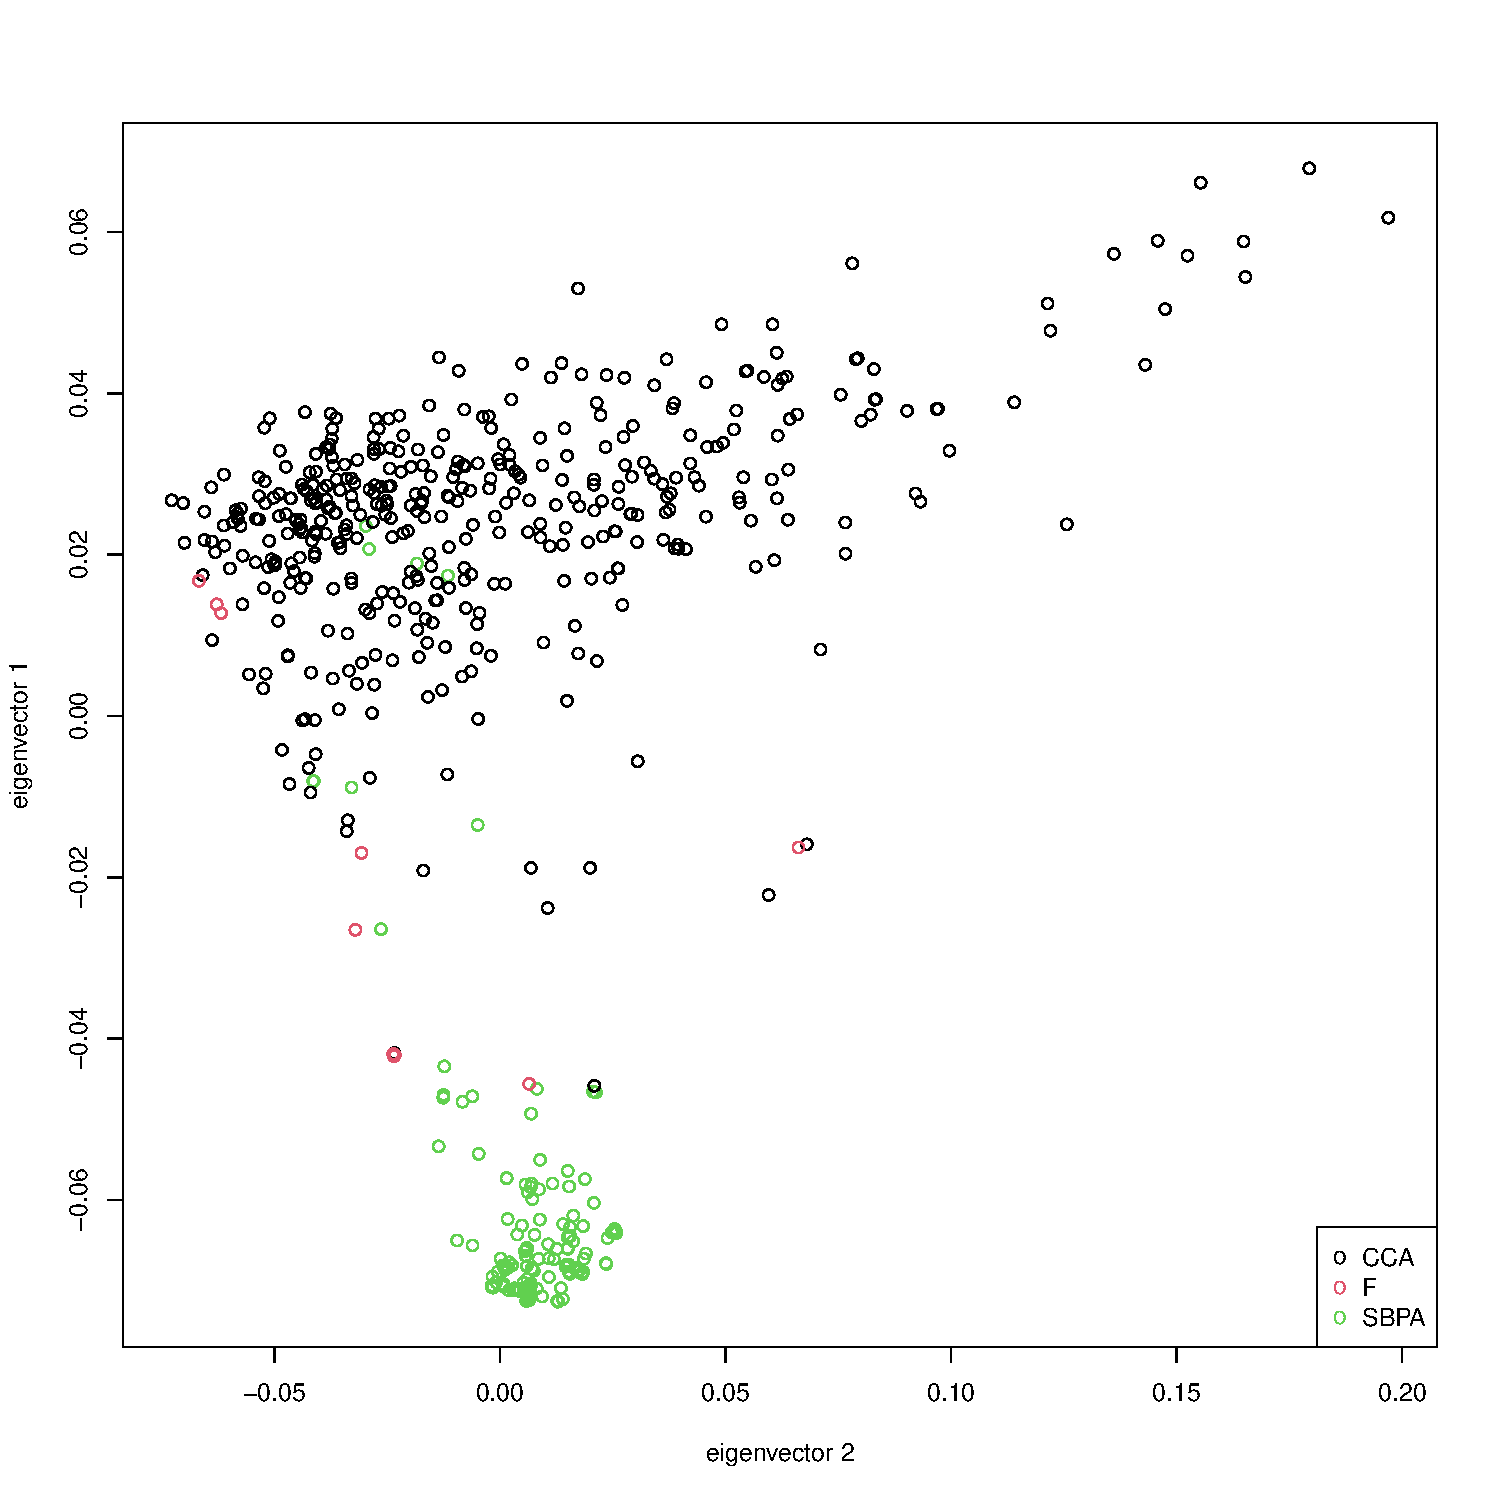
\includegraphics[width=\linewidth]{plot_PCA_origin.pdf}
\caption{Principal component analysis for soybean samples from defined groups, Core collection Accessions (CCA) in black, the Swedish Breeding Program Accessions (SBPA) in green and the Founders of the breeding progran (F) in red.}%
\label{fig:pca}
\end{figure}
\subsection{PCA2 figure}


Figure \ref{fig:pca2} .

\begin{figure}[t]
\centering
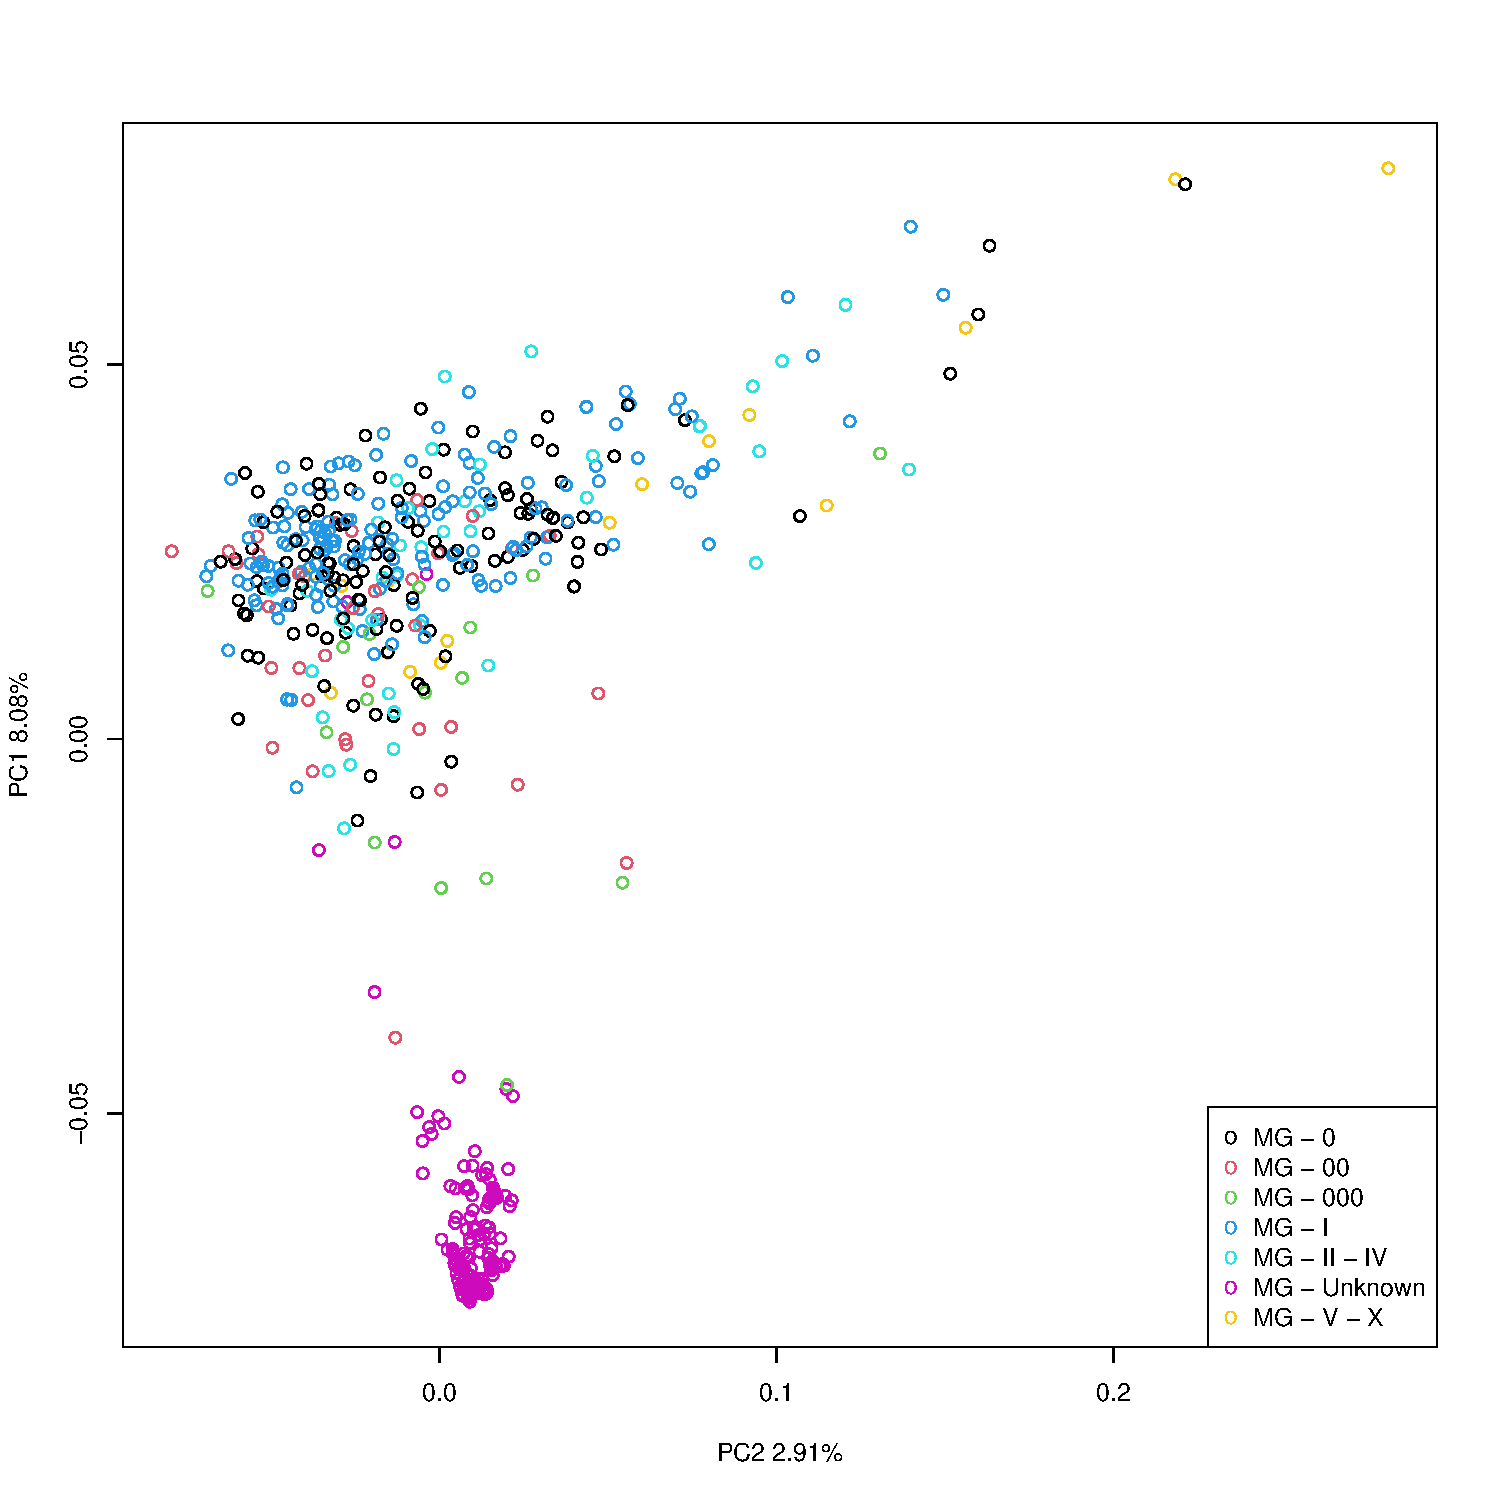
\includegraphics[width=\linewidth]{plot_PCA_mg1.pdf}
\caption{Principal component analysis for soybean samples from the whole genome sequence data, including the 155 Nordgen accessions and the 409 Core collection accessions. Indicated is the Maturity groups assigned to the accessions.}
\label{fig:pca2}
\end{figure}


\subsection{PCA3 figure}


Figure \ref{fig:pca3} .

\begin{figure}[t]
\centering
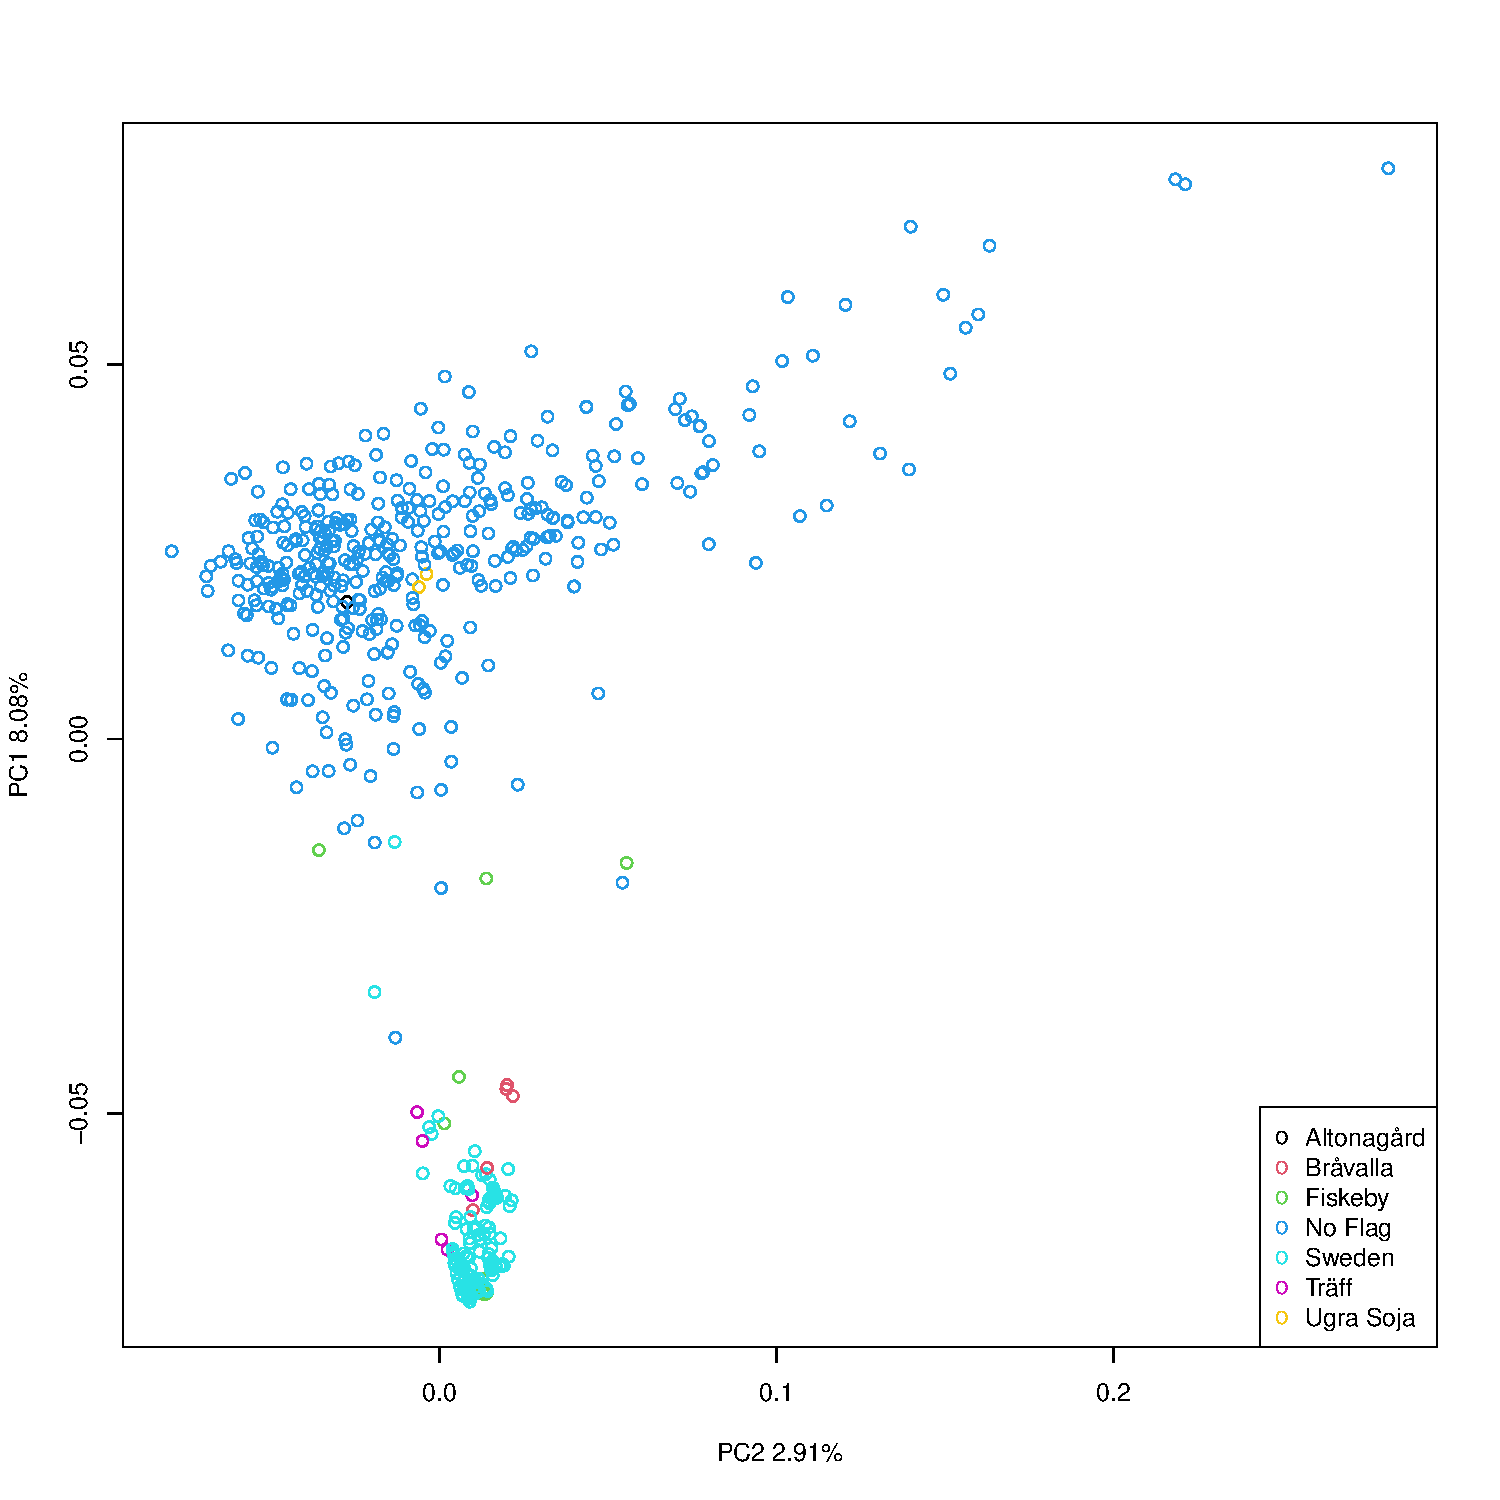
\includegraphics[width=\linewidth]{plot_PCA_flag.pdf}
\caption{PCA MG status}%
\label{fig:pca3}
\end{figure}
\subsection{Dendogram figure}

Figure \ref{fig:dendo} shows an example figure.

\begin{figure}[t]
\centering
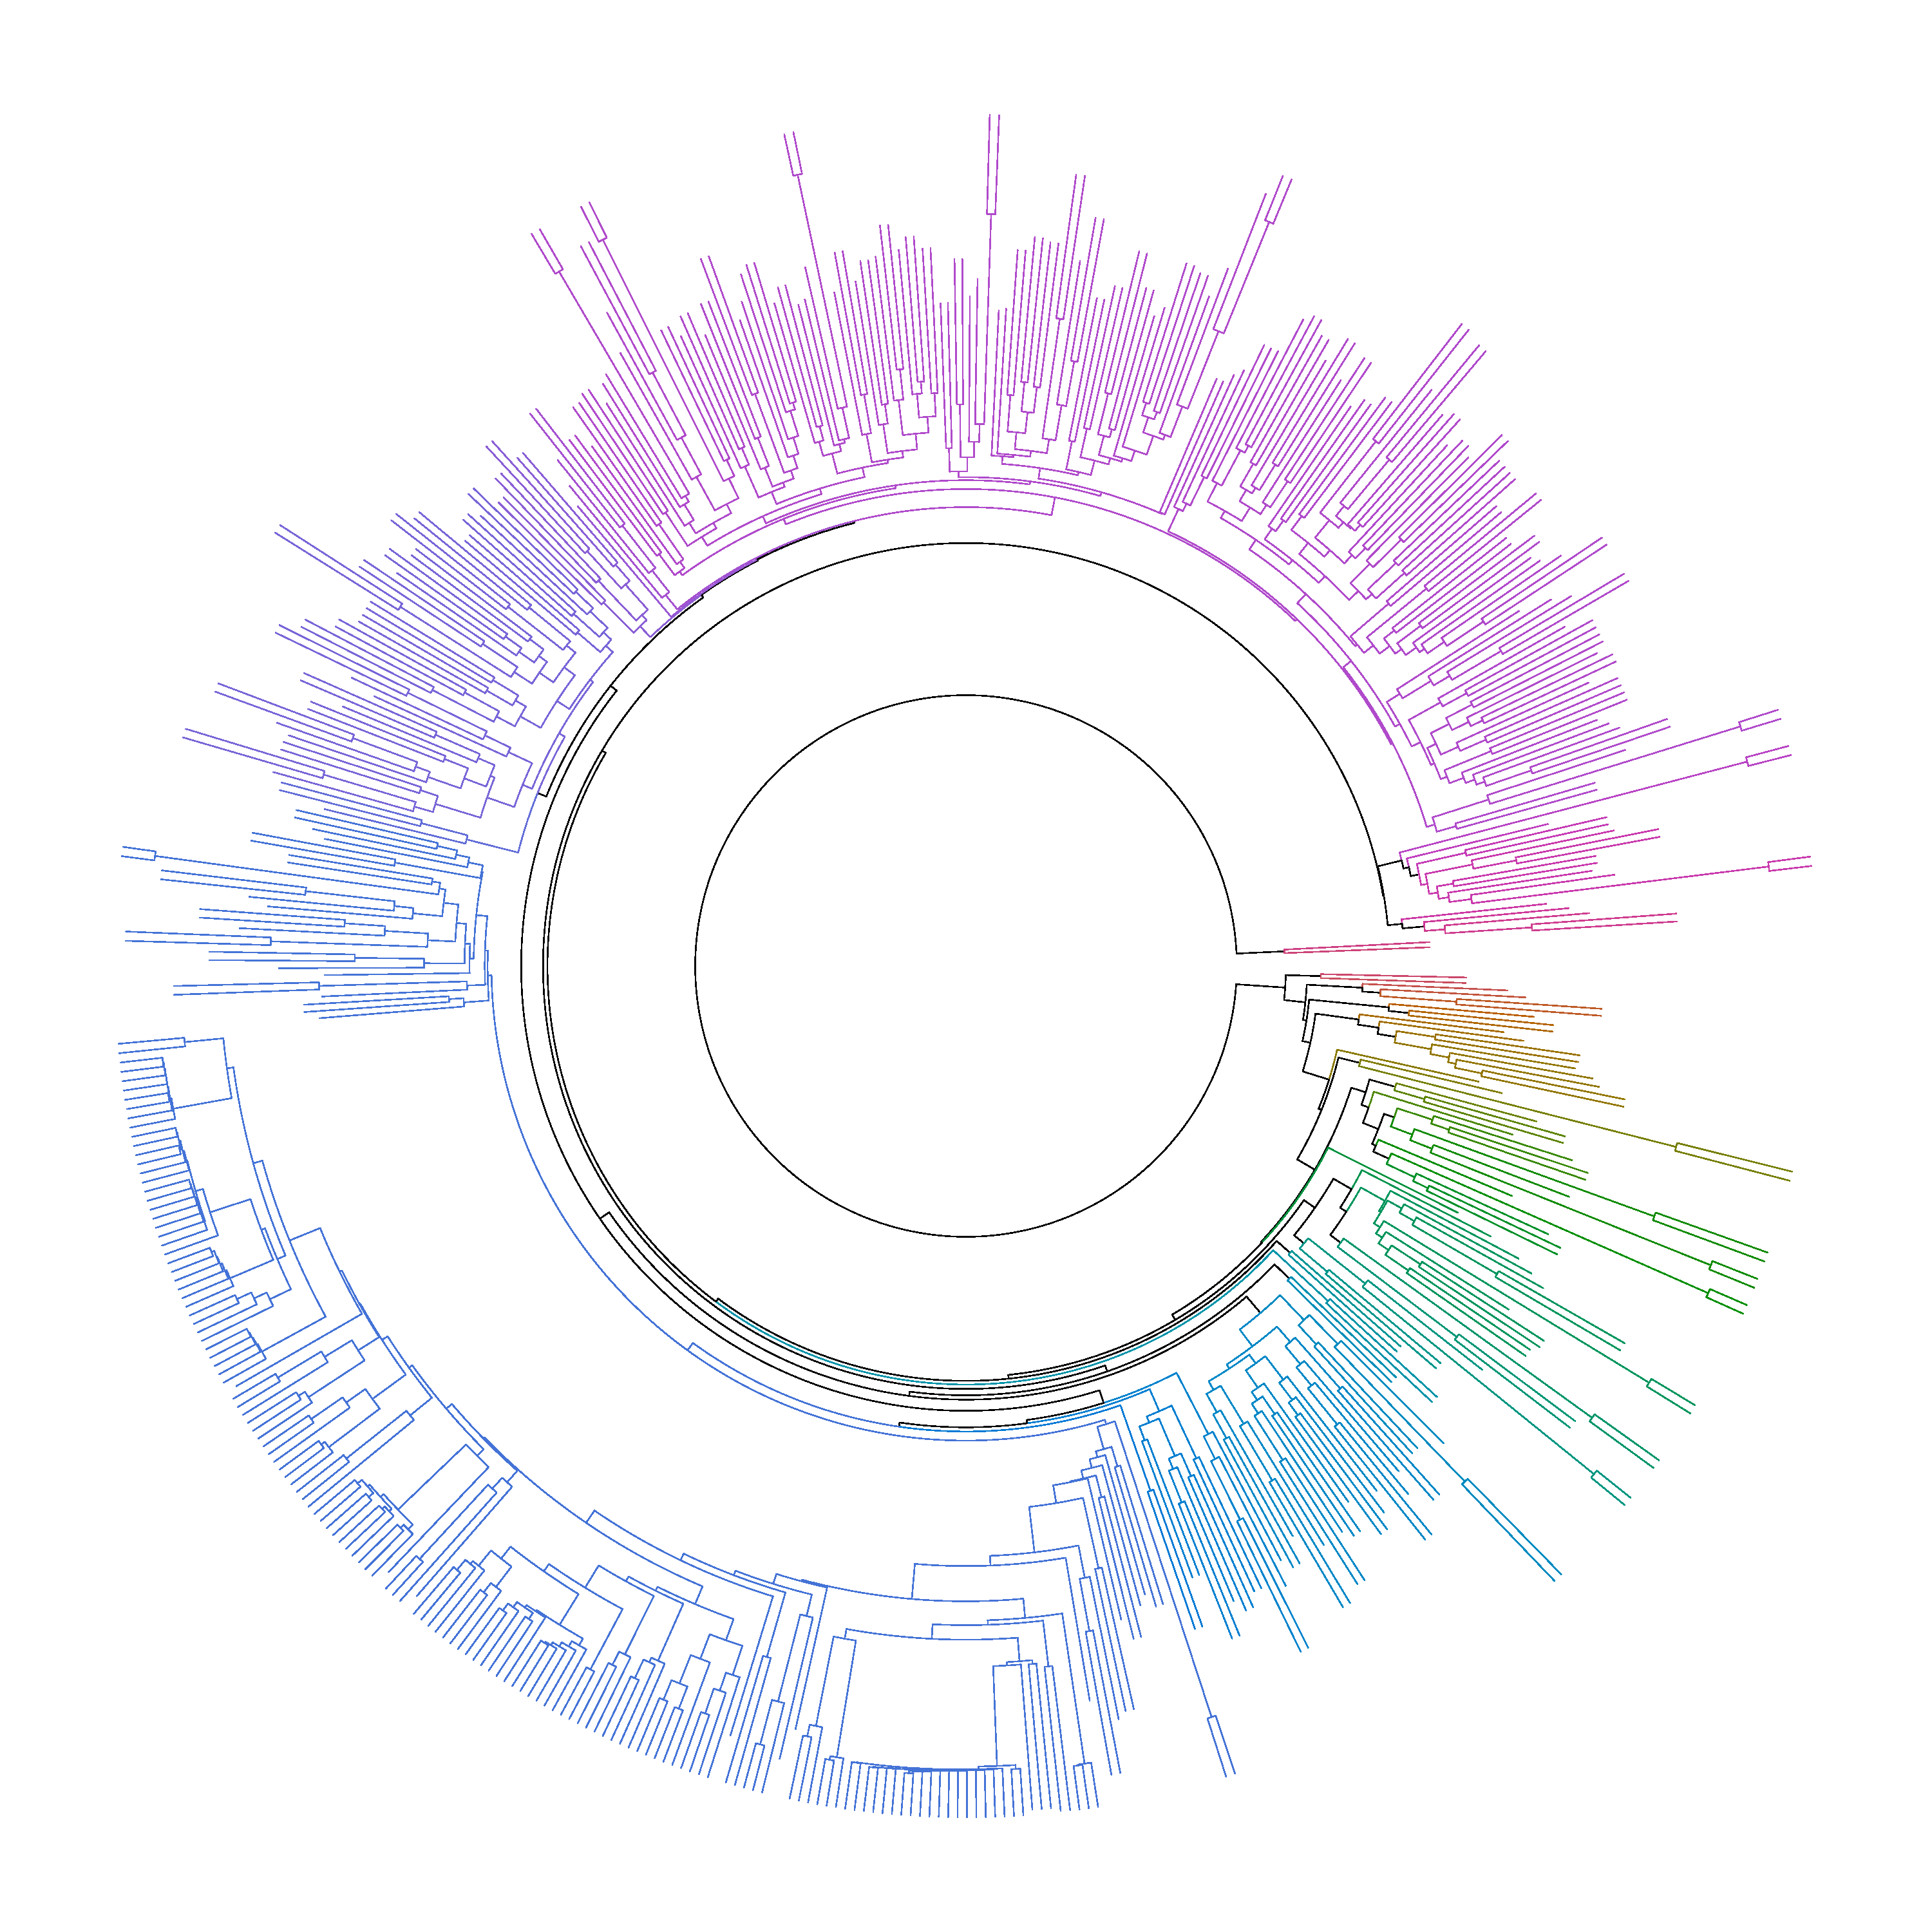
\includegraphics[width=\linewidth]{rainbow.pdf}
\caption{Hierarchical cluster dendrogram based on pairwise identity-by-state (IBS) values from SNP data for all samples. describe dendogram}%
\label{fig:pca}
\end{figure}

\subsection{Sample figure}

Figure \ref{fig:spectrum} shows an example figure.

\begin{figure}[t]
\centering
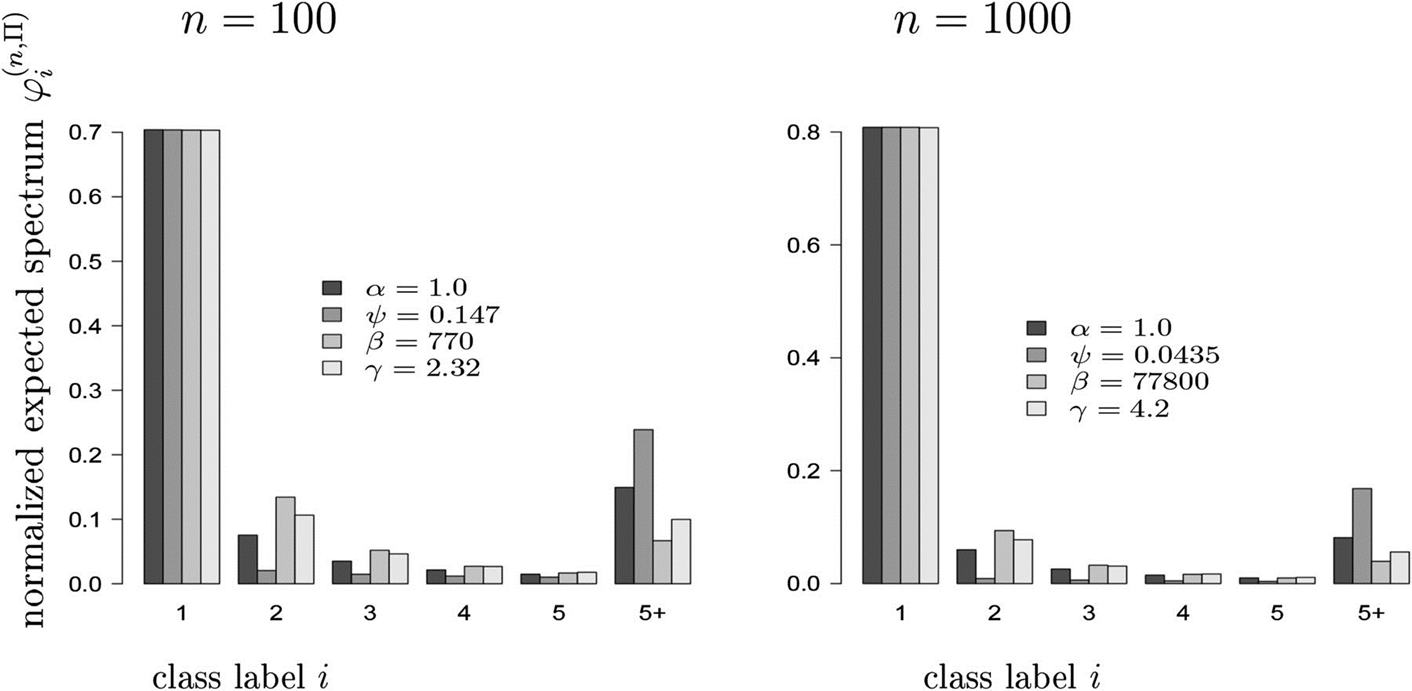
\includegraphics[width=\linewidth]{example-figure}
\caption{Example figure from \url{10.1534/genetics.114.173807}. Please include your figures in the manuscript for the review process. You can upload figures to Overleaf via the Project menu. Images of photographs or paintings can be provided as raster images. Common examples of raster images are .tif/.tiff, .raw, .gif, and .bmp file types. The resolution of raster files is measured by the number of dots or pixels in a given area, referred to as “dpi” or “ppi.”
\begin{itemize}
\item  minimum resolution required for printed images or pictures: 350dpi
\item  minimum resolution for printed line art: 600dpi (complex or finely drawn line art should be 1200dpi)
\item minimum resolution for electronic images (i.e., for on-screen viewing): 72dpi
\protect\end{itemize}
Images of maps, charts, graphs, and diagrams are best rendered digitally as geometric forms called vector graphics. Common file types are .eps, .ai, and .pdf. Vector images use mathematical relationships between points and the lines connecting them to describe an image. These file types do not use pixels; therefore resolution does not apply to vector images.
Label multiple figure parts with A, B, etc. in bolded. Legends should start with a brief title and should be a self-contained description of the content of the figure that provides enough detail to fully understand the data presented. All conventional symbols used to indicate figure data points are available for typesetting; unconventional symbols should not be used. Italicize all mathematical variables (both in the figure legend and figure) , genotypes, and additional symbols that are normally italicized.}%
\label{fig:spectrum}
\end{figure}

%\begin{figure}[htbp]
%\centering
%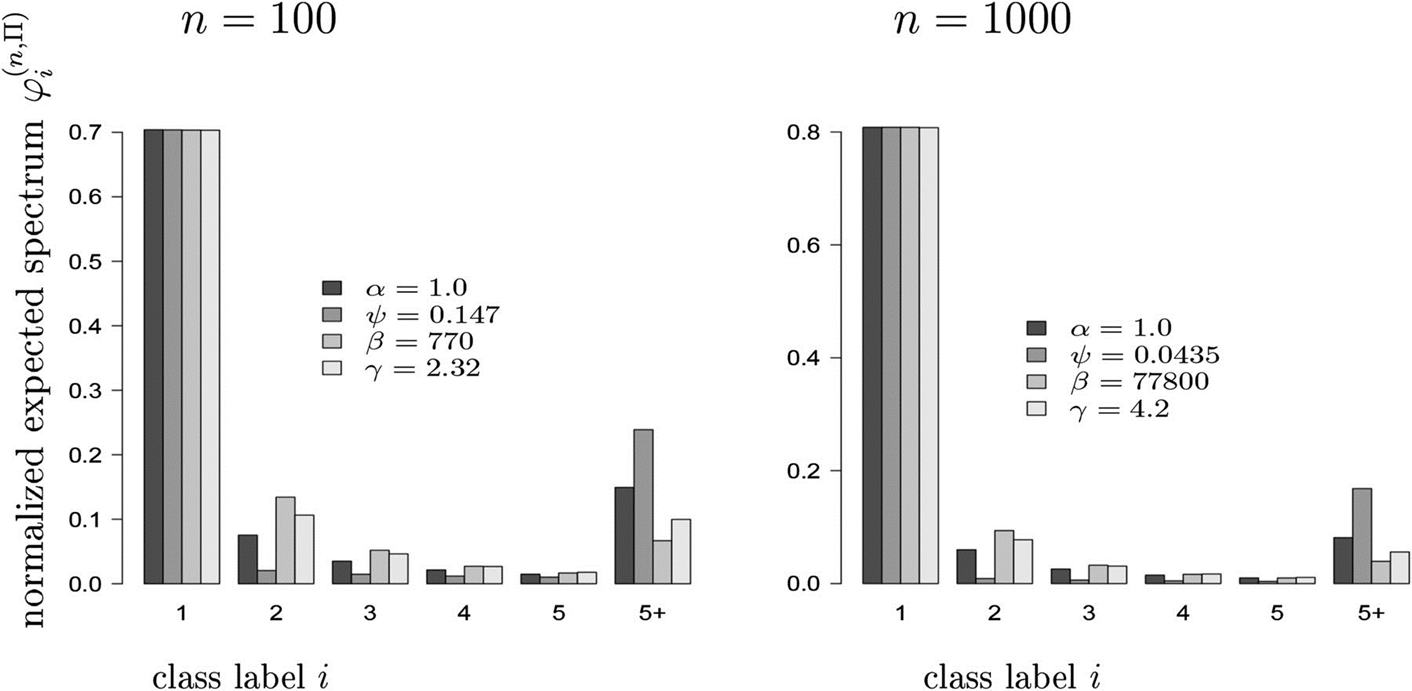
\includegraphics[width=\linewidth]{example-figure}
%%\caption{Example movie (the figure file above is used as a placeholder for this example). \textit{GENETICS} supports video and movie files that can be linked from any portion of the article - including the abstract. Acceptable formats include .asf, avi, .wav, and all types of Windows Media files.
%%}%
%%\label{video:spectrum}
%\end{figure}

Figures and Tables should be labelled and referenced in the standard way using the \verb|\label{}| and \verb|\ref{}| commands.

\subsection{Sample table}

Table \ref{tab:shape-functions} shows an example table. Avoid shading, color type, line drawings, graphics, or other illustrations within tables. Use tables for data only; present drawings, graphics, and illustrations as separate figures. Histograms should not be used to present data that can be captured easily in text or small tables, as they take up much more space.

Tables numbers are given in Arabic numerals. Tables should not be numbered 1A, 1B, etc., but if necessary, interior parts of the table can be labeled A, B, etc. for easy reference in the text.

\begin{table*}[p]
\centering
\caption{Students and their grades}
\begin{tableminipage}{\textwidth}
\begin{tabularx}{\textwidth}{@{}XXXX@{}}
\hline
{\bf Student} & {\bf Grade}\footnote{This is an example of a footnote in a table. Lowercase, superscript italic letters (a, b, c, etc.) are used by default. You can also use *, **, and *** to indicate conventional levels of statistical significance, explained below the table.} & {\bf Rank} & {\bf Notes} \\
\hline
Alice & 82\% & 1 & Performed very well.\\
Bob & 65\% & 3 & Not up to his usual standard.\\
Charlie & 73\% & 2 & A good attempt.\\
\hline
\end{tabularx}
  \label{tab:shape-functions}
\end{tableminipage}
\end{table*}

\section{Sample equation}

Let $X_1, X_2, \ldots, X_n$ be a sequence of independent and identically distributed random variables with $\text{E}[X_i] = \mu$ and $\text{Var}[X_i] = \sigma^2 < \infty$, and let
\begin{equation}
S_n = \frac{X_1 + X_2 + \cdots + X_n}{n}
      = \frac{1}{n}\sum_{i}^{n} X_i
\label{eq:refname1}
\end{equation}
denote their mean. Then as $n$ approaches infinity, the random variables $\sqrt{n}(S_n - \mu)$ converge in distribution to a normal $\mathcal{N}(0, \sigma^2)$.

\section{Supplementary Material}
\label{sec:supplementary:material}
Supplementary Material Methods (S Methods)
\href{PCA.html}

\section{Data availability}

For example: Strains and plasmids are available upon request. File S1 contains detailed descriptions of all supplemental files. File S2 contains SNP ID numbers and locations. File S3 contains genotypes for each individual. Sequence data are available at GenBank and the accession numbers are listed in File S3. Gene expression data are available at GEO with the accession number: GDS1234. Code used to generate the simulated data can be found at \url{https://github.com/JosephineConnelly/soyadapt_data_analysis}.

\section{Acknowledgments}
Acknowledgments should be included here.

\section{Funding}
Funding, including Funder Names and Grant numbers should be included here.

\section{Conflicts of interest}
There are  no known conflicts of interest.

\section{In-text citations}

Add citations using the \verb|\citep{}| command, for example \citep{neher2013genealogies} or for multiple citations, \citep{neher2013genealogies, rodelsperger2014characterization,Falush16}


\bibliography{bibliography}


\end{document} 